%%%%%%%%%%%%%%%%%%%%%%%%%%%%%%%%%%%%%%%%%%%%%%%%%%%%%%%%%%%%%%%%%
% !TEX root = interimreport.tex
\clearpage
\chapter{RISC-V}\label{ch:riscv}
%%%%%%%%%%%%%%%%%%%%%%%%%%%%%%%%%%%%%%%%%%%%%%%%%%%%%%%%%%%%%%%%%
In this project, our target is a 32-bit RISC-V core. RISC stands for reduced instruction set computer and RISC-V is an open standard Instruction Set Architecture. \cite{riscvorgabout} It is structured as a small base instruction set architecture and it has different additional extensions. The base instruction set architecture (ISA) is straightforward, rendering RISC-V appropriate for academic and learning purposes, yet extensive enough to function as a cost-effective and energy-efficient ISA for embedded systems \cite{watermanriscv}. Being open-source and royalty-free is another significant advantage and is an important reason why RISC-V is being commonly used. 
RISC-V was developed by Prof. Krste Asanović and his students Andrew Waterman and Yunsup Lee. They started working on this project in 2010 as a part of as part of the Parallel Computing Laboratory which was in UC Berkeley. Par Lab was sponsored by several companies and worked on advancing parallel computing.

\section{RISC-V ISA}
The Instruction Set Architecture (ISA) constitutes a part of a computer’s abstract design that defines how the CPU is managed by the software. It serves as a bridge between the software and hardware, defining the processor’s abilities and the methods by which it performs tasks. Its level in the system can be seen in Figure \ref{fig:level_of_abstraction_diagram}.

\begin{figure}[h!]
    \centering
    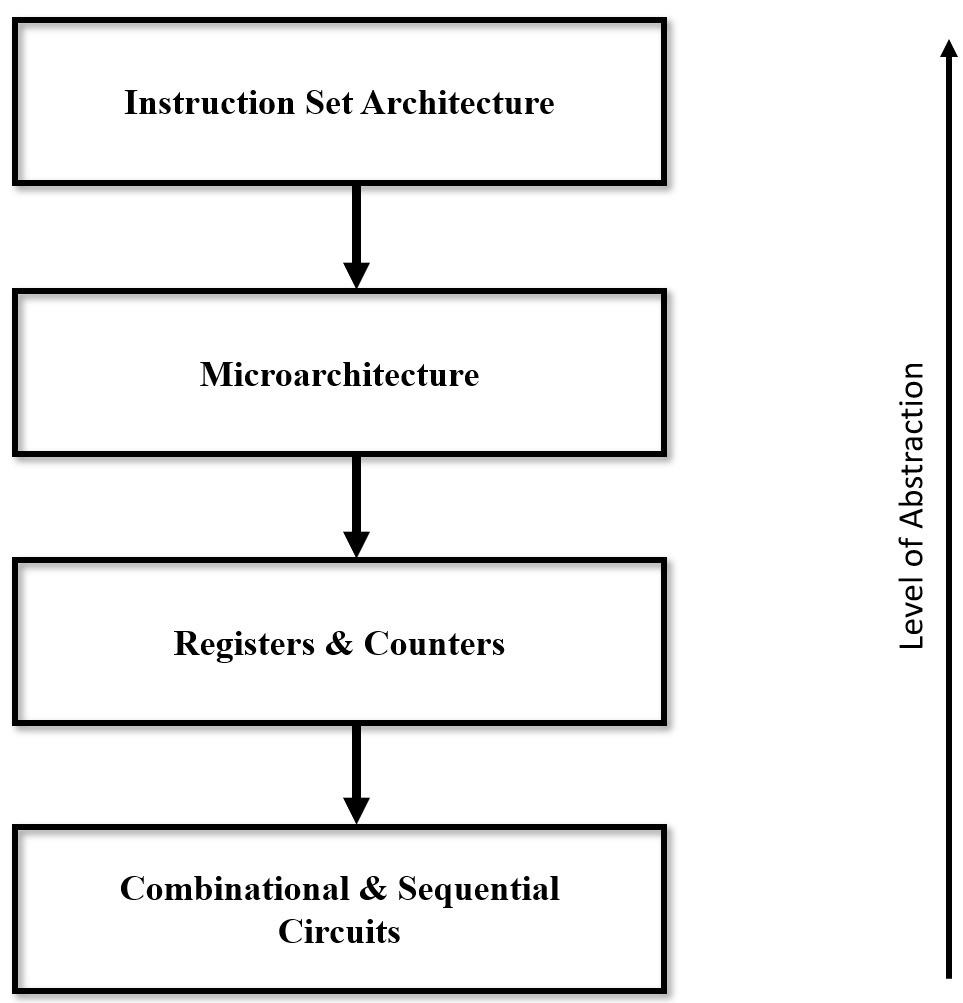
\includegraphics[scale=0.25]{riscv/level_of_abstraction_diagram.jpeg}
    \caption{Level of abstraction diagram \cite{levelofabstrac}}
    \label{fig:level_of_abstraction_diagram}
\end{figure}

There are different base integer variants of RISC-V such as RV32I, RV64I, and RV128I. These have address spaces of 32, 64, and 128 bits respectively \cite{Altinayozlem}. In our project, we are interested in 32-bits. RISC-V has 32 general-purpose registers. Their application binary interface names and purposes can be seen in Figure \ref{fig:riscv_registers}. Also in the Figure, we can see a different set of registers. These registers are used for floating point operations. Their ABI and purposes are also given.

\begin{figure}[h!]
    \centering
    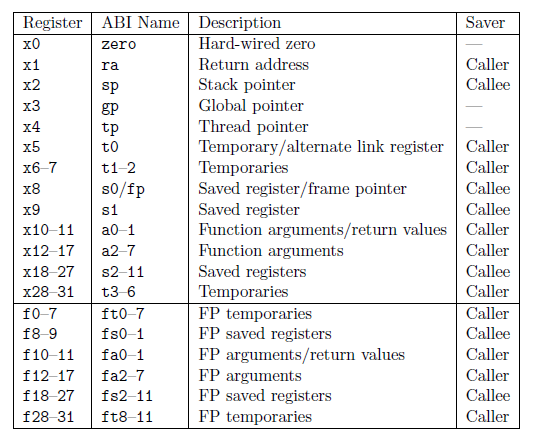
\includegraphics{riscv/riscv_registers.png}
    \caption{RISC-V registers \cite{rvregisters}}
    \label{fig:riscv_registers}
\end{figure}

\section{RISC-V Base Instructions}
There are four basic instruction formats in the base RV32I ISA. These are named R, I, S, U and all of these are 32-bits in length. There are two more additional variants named B and J as well \cite{rvmanual}. These formats are given in Figure \ref{fig:risc-v_base_instruction_formats}.
\begin{figure}
    \centering
    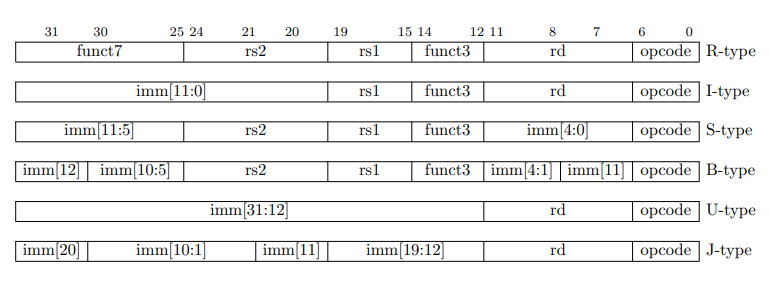
\includegraphics{riscv/riscv_base_instruction_formats.png}
    \caption{RISC-V base instruction formats \cite{rvmanual}}
    \label{fig:risc-v_base_instruction_formats}
\end{figure}

$R_{S1}$ and $R_{S2}$ are the source registers and $R_d$ is the destination register. An immediate value can also be used in some of the formats. 
The base instructions of the RV32I are given in Figure \ref{fig:rv32i_base_instruction_set}. By inspecting their formats, we can see which type the instructions belong to. For example, the ADDI instruction is an I-type instruction and XOR is an R-type instruction.

\begin{figure}[h!]
    \centering
    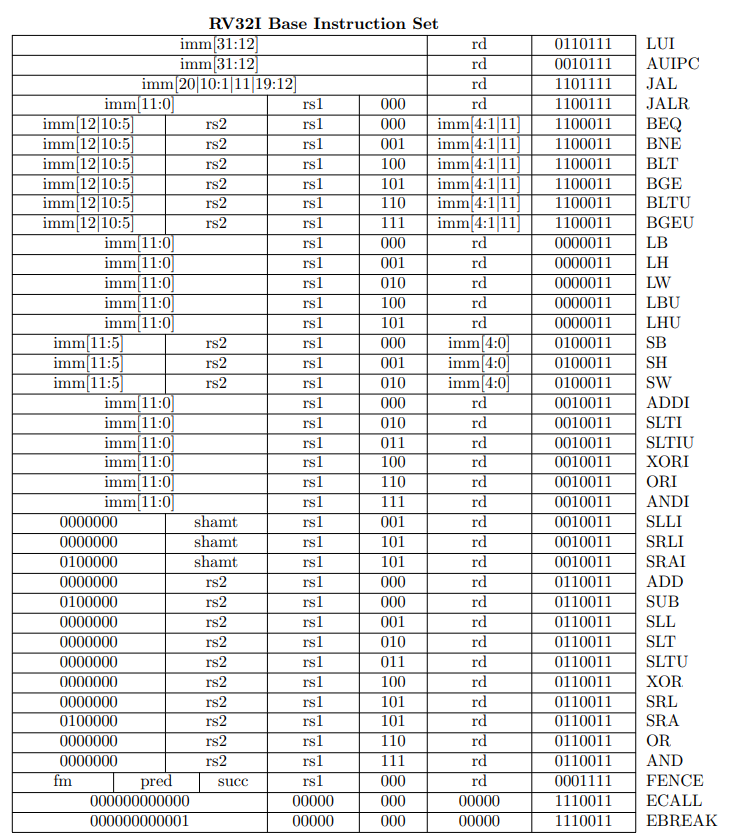
\includegraphics{riscv/rv32i_base_instruction_set.png}
    \caption{RV32I base instruction set \cite{rvmanual}}
    \label{fig:rv32i_base_instruction_set}
\end{figure}

\section{RISC-V Extensions}
We had mentioned the extensions previously. Abbreviations for these extensions and what they are for are given in Figure \ref{fig:list_of_standard_extension_sets}.
\begin{figure}[h!]
    \centering
    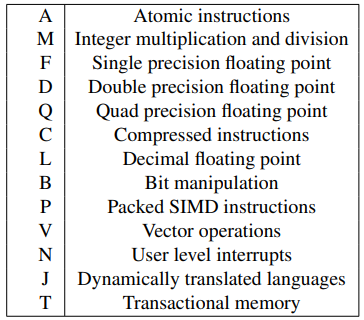
\includegraphics{riscv/list_of_standard_extension_sets.png}
    \caption{List of standard extension sets \cite{erfan}}
    \label{fig:list_of_standard_extension_sets}
\end{figure}

Thanks to these instruction extensions, more specific tasks can be implemented since we are not limited by the base instructions.
Among these, the bit manipulation (B) standard extension containining numerous instructions that can be useful in a wide range of applications. This extension's instructions mainly operate on the bits. These extensions are also divided into several groups according to common properties. These subgroups and their purposes can be seen in Figure \ref{fig:bit_manipulation_extension_groupings}.
\begin{figure}[h!]
    \centering
    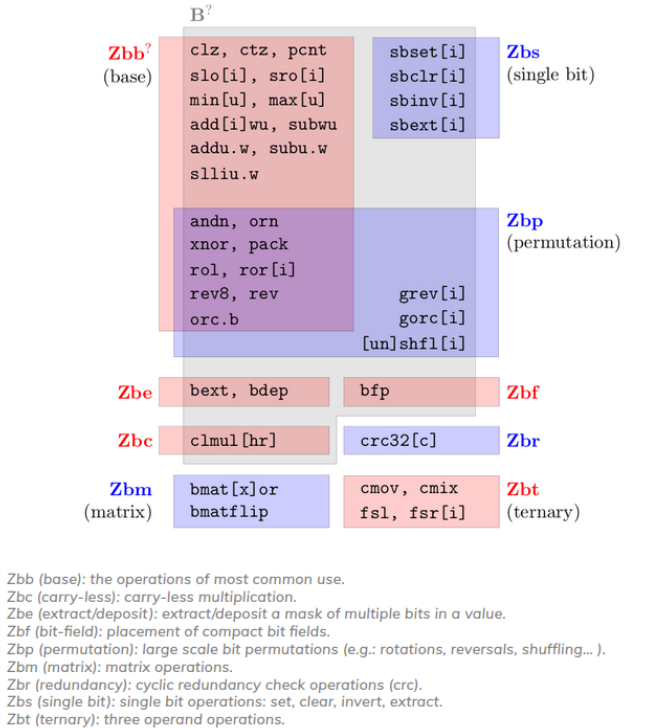
\includegraphics{riscv/bit_manipulation_extension_groupings.png}
    \caption{Bit manipulation extension groupings \cite{bitmanipgroups}}
    \label{fig:bit_manipulation_extension_groupings}
\end{figure}

Grouping these instructions according to how commonly they are used and the similarity of the operations that they perform makes them more organized and easier to work on with hardware and software. 
Some of these extensions are compatible with RV64 only. The compatibilities and the groups the instructions belong to are given in Figure \ref{fig:rv32_rv64_compatibilities_and_groups}.
\begin{figure}[h!]
    \centering
    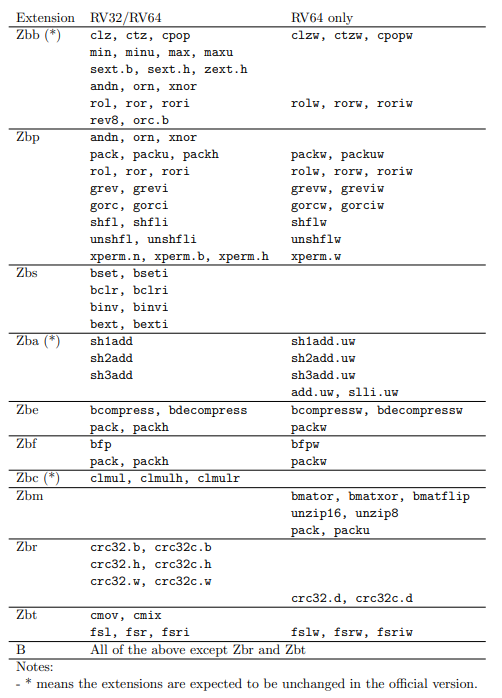
\includegraphics{riscv/rv32_rv64_compatibilities_and_groups.png}
    \caption{Bit RV32/RV64 compatibilities and groups \cite{bitmanipdraft}}
    \label{fig:rv32_rv64_compatibilities_and_groups}
\end{figure}

\clearpage

To give a clearer image of what bit manipulation (B) instructions do, a few of them will be explained. For example, “CLZ” is an instruction for counting the leading zeros. Its purpose is to find out how many zeros are there before encountering a 1, starting from the most significant bit. Another example is “ORN” instruction. It negates the second operand and performs bitwise or with the first one. 
\par
Zba is also a subgroup of the bit manipulation extensions. Shift and add instructions are included in this group and they perform a left shift by 1, 2, or 3 bits since they are commonly used in codes and also because they require only a minimal amount of extra hardware beyond that of a basic adder. This way, lengthening the critical path in implementations can be avoided. For example, SH1ADD is a part of this group and it shifts the operand by 1 and adds 1 \cite{bitmanipulationisaextensions}.
\par
There is also a scalar cryptography instruction set extension for RISC-V. The RISC-V Scalar Cryptography extensions allow cryptographic tasks to be completed more quickly. Furthermore, these extensions significantly reduce the difficulty of implementing fast and secure cryptography in embedded devices and IoT \cite{cryptogroups}. This instruction set extension is also divided into subgroups according to the purpose and similarity of the instructions. The groups are given in Figure \ref{fig:cryptography_extension_subgroups}. These groups and their purposes can be explained briefly.

\begin{itemize}
    \item Zbkb contains bit manipulation instructions for cryptography. These are a selection of the bit manipulation extension Zbb that have specific applications in cryptography. 
    \item Zbkc contains carry-less multiply instructions.
    \item Zbkx instructions can be useful for implementing s-boxes in constant time.
    \item Zknd contains instructions that help speed up the decryption and key schedule functions of the AES block cipher and Zkne does the same for encryption.
    \item Zknh has some instructions that can help speed up the SHA2 family of cryptographic hash functions.
    \item Zksed contains instructions that speed up the SM4 block cipher.
    \item Zksh instructions help accelerate the SM3 hash function.
    \item Zkr can be useful to seed cryptographic random bit generators \cite{cryptoextensiondoc}.
\end{itemize}

These extensions are supported by the compiler but pattern matching support for Zbkb and Zbkx is incomplete in LLVM RISC-V backend. Also for Zknd, Zkne, Zknh, Zksed and Zksh, no pattern matching exists. Therefore, these instructions can be only used via builtin functions or from the assembler \cite{llvmextensionspage}.

\begin{figure}
    \centering
    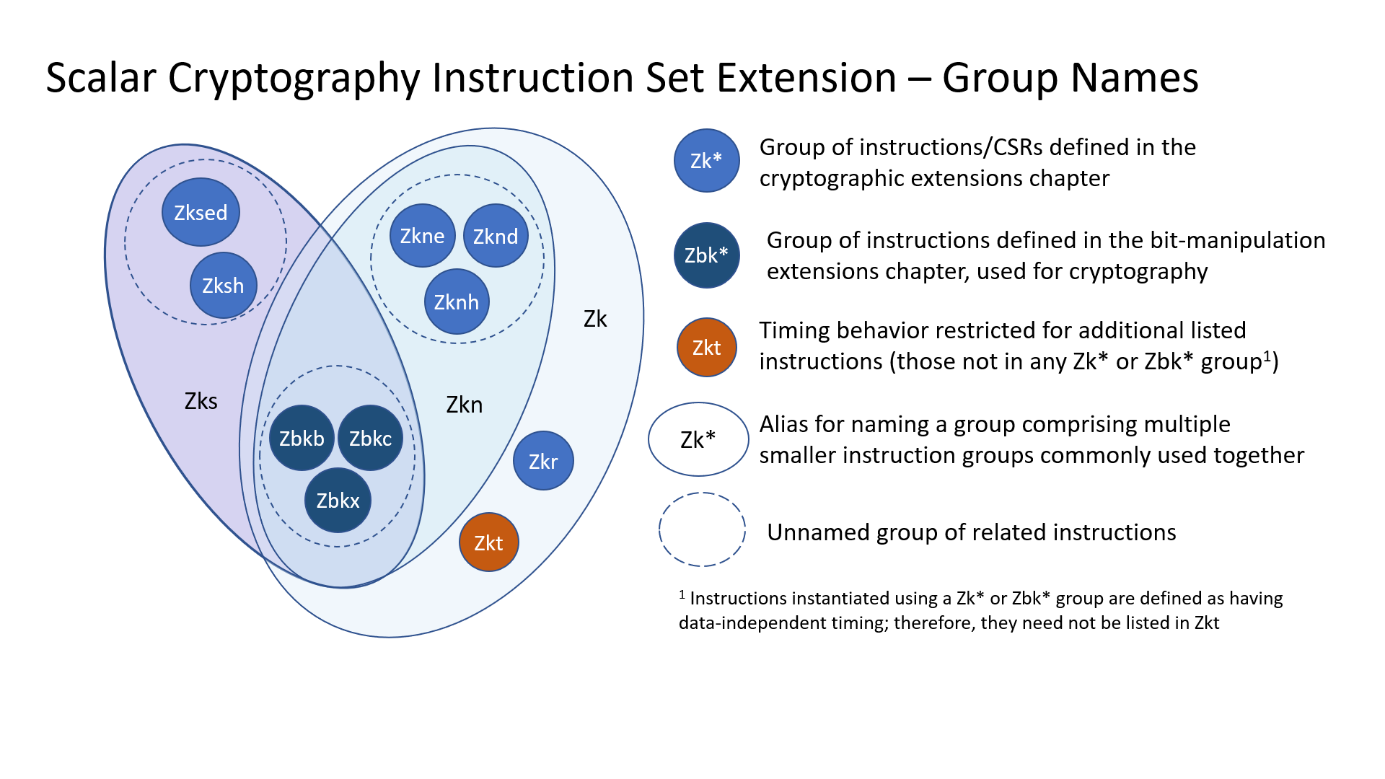
\includegraphics{riscv/cryptography_extension_subgroups.png}
    \caption{Cryptography extension subgroups \cite{cryptogroupsdiag}}
    \label{fig:cryptography_extension_subgroups}
\end{figure}

The modular structure of these extensions is useful for hardware and software developers. For example the B extension is built in Clang so only an extra argument will provide the necessary instructions from the input extension.

It is important for hardware developers to consider that developing accelerators targeting instructions in standard extensions will reduce the software workload significantly. The reason for this is LLVM supports RISC-V standard extensions and follows updates closely. Corner cases are thought out and optimization opportunities are utilized. RISC-V standard extensions are comprehensive and may already contain the extensions that we want to implement. After making sure that the extension we want is not present, we may try to implement non-standard extensions.
